\section{Deformable DETR: Deformable Transformers for End-to-End Object Detection}

\label{appendix:deformable-detr-paper}

\subsection{Overview}

\par Zhu \textit{et al} in their 2021 paper titled \textit{Deformable DETR: Deformable Transformers} for End-to-End Object Detection aims to replace the vanilla dense attention, which is the main computational bottleneck in DETR, with a deformable attention module. This can significantly reduce computational costs while also improving convergence \cite{zhu2020deformable}. 
\par

\subsection{Architecture}
\begin{figure}[h]
	\centering
	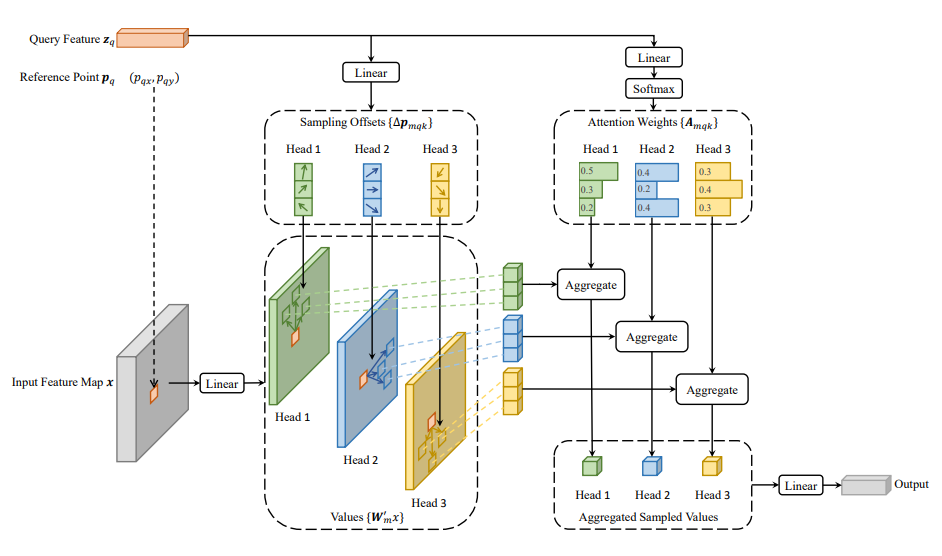
\includegraphics[width=\linewidth]{assets/img/deformable-attention-module.png}
	\caption{Deformable Attention Module by Zhu
		\textit{et al} (Courtesy \cite{zhu2020deformable})}
\end{figure}

\subsubsection{Deformable Attention Module} 
\begin{itemize}
	\item It attends to only a small set of key sampling points around a reference point, regardless of the spatial size of the feature maps. By assigning only a small fixed number of keys for each query, the issues of convergence and feature spatial resolution can be mitigated.
	\item Given an input feature map $x \in R^{C\times H \times W}$ , let q index a query element with content feature zq and a 2-d reference point pq, the deformable attention feature is calculated by
	$$ DeformAttn(z_q, p_q, x) = \displaystyle\sum\limits_{m=1}^M W_m
	[\displaystyle\sum\limits_{k=1}^K A_{mqk}\cdot W'_mx(p_q+\Delta p_{mqk})]
	$$
	where k indexes the sampled keys, m indexes the attention head, and K is the total sampled key number. $\Delta p_{mqk}$ and $A_{mqk}$ denote the sampling offset and attention weight of the $k^{th}$ sampling point in the $m^{th}$ attention head, respectively.
\end{itemize}

\subsubsection{Multi-scale Deformable Attention Module}
\begin{itemize}
	\item Deformable attention module can be easily extended for multi-scale feature maps.  
	\item Let $\{{x^l}\}_{l=1}^L$ be the input multi-scale feature maps, where  $x^l \in R^{C\times H^l \times W^l}$ . Let $ \hat p_q \in [0, 1]^2$ be the normalised coordinates of the reference point for each query element q, then the multi-scale deformable attention module is applied as 
	$$DeformAttn(z_q, \hat{p}_q, \{{x^l}\}_{l=1}^L) = 
	\displaystyle\sum\limits_{m=1}^M W_m
	[\displaystyle\sum\limits_{l=1}^L\displaystyle\sum\limits_{k=1}^K A_{mlqk}\cdot W'_mx^l(\phi _l (\hat p_q)+\Delta p_{mlqk})]$$
	
	where l indexes the input feature level, m indexes the attention head, and k indexes the sampling point. $\Delta p_{mlqk}$ and $A_{mlqk}$ denote the sampling offset and attention weight of the kth sampling point in the lth feature level and the mth attention head, respectively
\end{itemize}

\subsubsection{Deformable Transformer Encoder}
\begin{itemize}
	\item The proposed multiscale deformable attention module replaces the transformer attention modules that process feature maps in DETR.
	\item The encoder's input and output are both multi-scale feature maps with the same resolutions.
\end{itemize}	


\subsubsection{Deformable Transformer Decoder}

\begin{itemize}
	\item The decoder includes cross-attention and self-attention modules.
	\item Object queries in the cross attention modules extract features from feature maps, where the key elements are from the encoder's output feature maps. Object queries interact with each other in the self-attention modules, where the key elements are of the object queries.
	\item Because the proposed deformable attention module is intended to process convolutional feature maps as key elements, the cross-attention module is replaced with the multi-scale deformable attention module, while the self-attention modules remain unaltered.
\end{itemize}
\subsection{Conclusion}
\par Zhu \textit{et al} present Deformable DETR \cite{zhu2020deformable}, an efficient and fast-converging end-to-end object detector.  The multi-scale deformable attention modules, which are an efficient attention mechanism in processing image feature maps, are at the core of Deformable DETR.